\documentclass[oneside, final, 14pt]{extreport}
\usepackage[utf8]{inputenc}
\usepackage[russian]{babel}
\usepackage{vmargin}
\setpapersize{A4}
\setmarginsrb{2cm}{1cm}{1cm}{1cm}{0pt}{0mm}{0pt}{13mm}
\usepackage{indentfirst}
\usepackage{amsmath}
\usepackage{graphicx}
\usepackage{wrapfig}
\sloppy

\begin{document}

\setcounter{chapter}{6}
\chapter{Динамическая обработка сигналов}
\tableofcontents

\section{Основные понятия}
\textbf{Динамическая обработка звука}~--- обработка, которая приводит к изменению динамического диапазона фонограммы.

Под \textbf{динамическим диапазоном сигнала} понимают отношение максимального и минимального уровней громкости (\emph{maximum}, \emph{minimum RMS power}).

Из всех процессов, используемых в создании музыки, динамическая обработка звука является, пожалуй, наиболее сложной для восприятия. В первую очередь это связано с тем, что зачастую результат обработки звука едва различим на слух~--- особенно для начинающих. Другая трудность заключается в количестве изменяемых параметров: их не так мало, и к тому же, изменение каждого из них не всегда приводит к очевидным результатам.

Динамические диапазоны музыкальных и речевых акустических сигналов разных типов, измеренные с помощью приборов, составляют в среднем:
\begin{itemize}
  \item 80 дБ для симфонического оркестра;
  \item 45 дБ для хора;
  \item 35 дБ для эстрадной музыки и солистов-вокалистов;
  \item 25 дБ для речи дикторов.
\end{itemize}


При записи уровни громкости необходимо регулировать, так как исходные (необработанные) сигналы зачастую имеют слишком большой динамический диапазон (например, до 80 дБ у симфонической музыки), а в домашних условиях аудио программы могут прослушиваться в диапазоне не более 40 дБ.

Динамический диапазон сигнала нужно согласовывать с динамическими диапазонами устройств записи, усиления и передачи. Для увеличения дальности действия FM-радиостанций динамический диапазон аудио сигнала нужно сжимать. Для снижения уровня шума в паузах динамический диапазон желательно увеличивать.

Мода, диктующая свои условия во всех сферах человеческой деятельности, в том числе и в звукозаписи, требует насыщенного, плотного звучания современной музыки, которое достигается резким сужением ее динамического диапазона.  В классической музыке важны нюансы, танцевальная музыка должна быть "сильнодействующей". На рис. представлена сигналограмма фрагмента оперы С. Рахманинова "<Алеко">, а на рис. ~--- сигналограмма современной танцевальной музыки. 

\begin{figure}[h!]
  \centering
  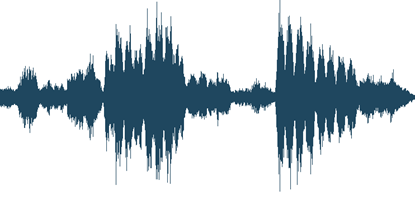
\includegraphics[width=0.75\textwidth]{pic-signal-01}
  \caption{Сигналограмма фрагмента оперы С. Рахманинова "<Алеко">}
  \label{pic-signal-01}
\end{figure}

\begin{figure}[h!]
  \centering
  
\includegraphics[width=0.75\textwidth]{pic-signal-02}
  \caption{Сигналограмма современной танцевальной музыки}
  \label{pic-signal-02}
\end{figure}

Любой инструмент динамической обработки имеет три функциональных элемента:
\begin{itemize}
  \item основной канал;
  \item детектор огибающей;
  \item контроллер громкости.
\end{itemize}

Задачи \textbf{детектора огибающей}~--- обнаружить момент пересечения аудио сигналом из основного канала порогового значения и измерить уровень аудио сигнала относительно данного по-рогового значения.

Задача \textbf{контроллера громкости}~--- выработать управляющее воздействие на основной канал в зависимости от измеренной величины аудио сигнала.

В зависимости от параметров контроллера громкости и детектора огибающей, различают следующие инструменты динамической обработки:
\begin{itemize}
  \item компрессор;
  \item экспандер;
  \item лимитер;
  \item автостабилизатор;
  \item шумоподавитель;
  \item устройства со сложным преобразованием динамического диапазона.
\end{itemize}

\section{Компрессор}
\textbf{Компрессор}~--- это инструмент динамической обработки, который уменьшает динамический диапазон сигнала и, благодаря этому, уменьшает разницу в уровне громкости между тихими и громкими звуками.

С помощью компрессора можно добиться более плотного и отчетливого звучания. На рис. представлен пример звука до (рис. \ref{pic-example-01}) и после обработки компрессором (рис. \ref{pic-example-02}).

\begin{figure}[h!]
  \centering
  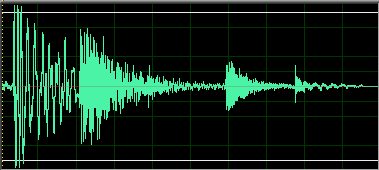
\includegraphics[width=0.75\textwidth]{pic-example-01}
  \caption{Сигналограмма исходного сигнала}
  \label{pic-example-01}
\end{figure}

\begin{figure}[h!]
  \centering
  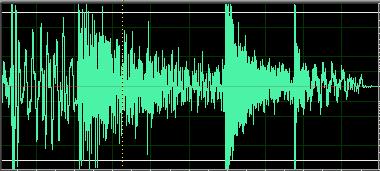
\includegraphics[width=0.75\textwidth]{pic-example-02}
  \caption{Сигналограмма сигнала после обработки компрессором}
  \label{pic-example-02}
\end{figure}

Результат динамической обработки зависит от правильного выбора значений нескольких основных параметров. К важнейшим из них относятся:
\begin{itemize}
  \item порог срабатывания (\emph{threshold});
  \item коэффициент компрессии (\emph{ratio});
  \item компенсирующее усиление (\emph{makeup gain});
  \item время атаки (\emph{attack time});
  \item время восстановления (\emph{release time}).
\end{itemize}

\textbf{Порог срабатывания} задает уровень громкости, при превышении которого начинается управление усилением. До тех пор, пока значение уровня сигнала меньше порогового, обработка не воздействует на сигнал. От величины порога зависит, коснется ли обработка только отдельных пиков, или сигнал будет подвергаться обработке постоянно. Если установить порог равным $0$ дБ, то динамической обработки происходить не будет.

На рис. \ref{pic-compress-01} представлена сигналограмма четырех коротких тональных сигналов разного уровня. Красной линией отмечен уровень порога компрессии. На рис. \ref{pic-compress-02} представлена сигналограмма сигнала после обработки компрессором.

\begin{figure}[h!]
  \centering
  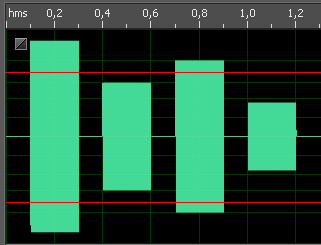
\includegraphics[width=0.5\textwidth]{pic-compress-01}
  \caption{Сигналограмма исходного сигнала}
  \label{pic-compress-01}
\end{figure}

\begin{figure}[h!]
  \centering
  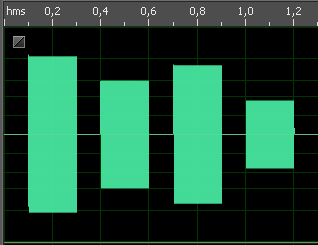
\includegraphics[width=0.5\textwidth]{pic-compress-02}
  \caption{Сигналограмма сигнала после обработки компрессором}
  \label{pic-compress-02}
\end{figure}

Сигналы №1 и №3 громче порога, поэтому они сжимаются. Сигналы №2 и №4 ниже порога, не изменяются. Кроме того, относительные громкости сигналов не изменяются.

\textbf{Коэффициент компрессии} определяет степень сжатия динамического диапазона сигнала, имеющего уровень выше порогового.
Например, коэффициент компрессии $2:1$ означает, что превышение входным сигналом порога на 2 дБ вызовет превышение порога выходным сигналом на 1 дБ. Абсолютному ограничению соответствует коэффициент компрессии "<$\inf:1$">, но на практике величины отношений больше, чем 20:1, дают такой же эффект. Чем больше коэффициент компрессии, тем меньше будет динамический диапазон обработанного сигнала. При коэффициенте сжатия 1:1 компрессии не будет вообще.

На рис. \ref{pic-compress-07} представлены Сигналограммы сигналов после обработки компрессором с коэффициентами 1:1, 2:1, 4:1, 8:1.

\begin{figure}[h!]
  \centering
  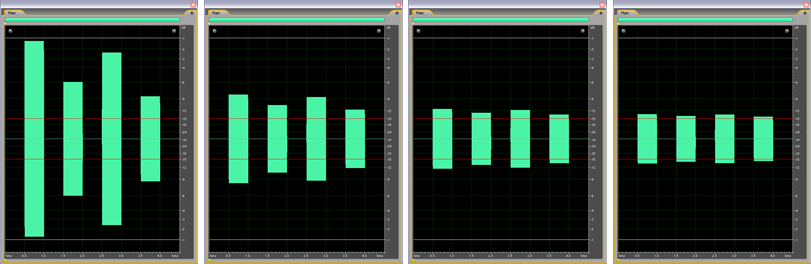
\includegraphics[width=0.95\textwidth]{pic-compress-07}
  \caption{Сигналограммы сигналов после обработки компрессором с коэффициентами 1:1, 2:1, 4:1, 8:1}
  \label{pic-compress-07}
\end{figure}

\textbf{Компенсирующее усиление} необходимо для того, чтобы усилить сигнал, который был ослаблен при выполнении динамической обработки. Чем больше степень сжатия, тем больше должно быть компенсирующее усиление. На рисунке \ref{pic-compress-03} приведена исходная запись и пример использования компрессии со степенью сжатия $2:1$, $4:1$, $8:1$.

\begin{figure}[h!]
  \centering
  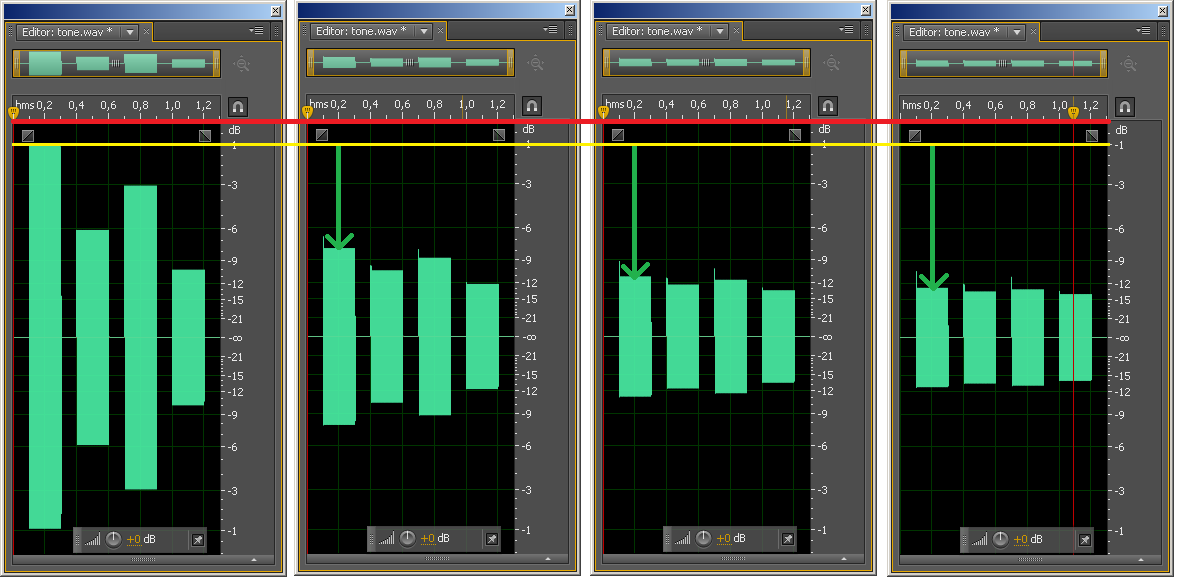
\includegraphics[width=0.95\textwidth]{pic-compress-03}
  \caption{Компрессия с коэффициентами 2:1, 4:1, 8:1}
  \label{pic-compress-03}
\end{figure}

Желтая линия обозначает максимальный уровень громкости исходного сигнала. Длина зеленой стрелки обозначает величину компенсирующего усиления, которое должно быть задано для того, чтобы после компрессии максимальный уровень громкости довести до максимального уровень громкости до компрессии.

Оценку инерционности устройств динамической обработки осуществляют на основе анализа двух временных характеристик: 
\begin{itemize}
  \item \textbf{время атаки} (\emph{attack time})~--- время реакция устройства на увеличение уровня сигнала;
  \item \textbf{время восстановления }(\emph{release time})~--- время реакция устройства на уменьшение уровня сигнала.
\end{itemize}

При больших времени атаки компрессору невозможно отслеживать резкие увеличения уровня входного сигнала, в результате в выходном сигнале будут присутствовать пики. Медленная атака менее склонна к искажениям, но неспособна реагировать на быстрые звуки. Если время атаки мало, то можно практически исключить возникновение пиков сигнала при скачкообразном увеличении его уровня. Быстрая атака может регулировать резкие переходы звука, но может вызывать искажения.

\begin{figure}[h!]
  \centering
  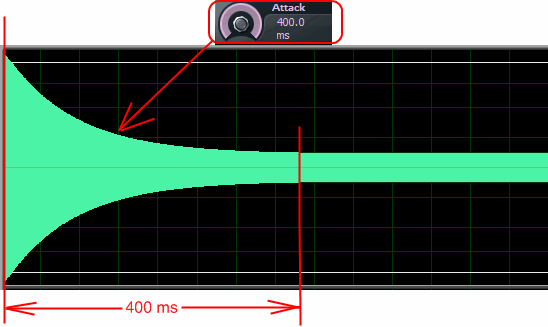
\includegraphics[width=0.75\textwidth]{pic-compress-04}
  \caption{Влияние времени атаки на форму сигнала}
  \label{pic-compress-04}
\end{figure}

На рис. \ref{pic-compress-05} продемонстрировано использование различных значений времени атаки. Первая огибающая является исходным сигналом, синусоидальной волной 1 кГц на -6 дБ, длительностью полсекунды. Три другие огибающие получены на выходе компрессора с порогом -20 дБ и степенью сжатия 10:1. Для второй огибающей время атаки компрессора равняется 0,05 мсек. Для третьей огибающей использовалось время атаки 1 мсек. Для четвертой огибающей использовалось время атаки 100 мсек.

\begin{figure}[h!]
  \centering
  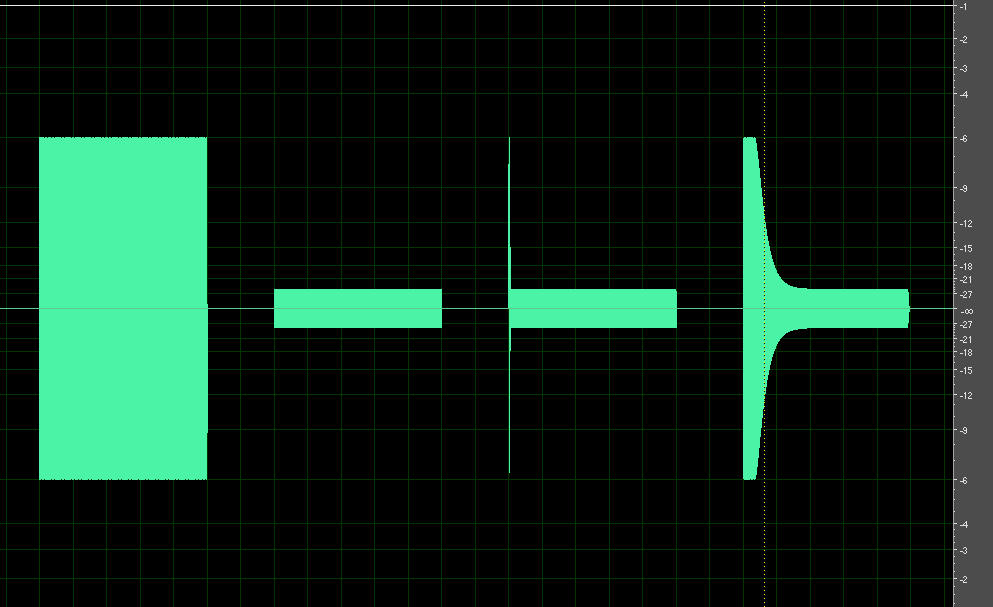
\includegraphics[width=0.75\textwidth]{pic-compress-05}
  \caption{Пример компрессии со временем атаки 0.05, 1 и 100 мсек}
  \label{pic-compress-05}
\end{figure}

\textbf{Время восстановления}~--- время, за которое устройство динамической обработки выходит из активного состояния после падения уровня сигнала ниже порогового. Если время восстановления слишком велико, то компрессор дольше находится в активном состоянии и воздействует на динамический диапазон даже тогда, когда это нежелательно (рис. \ref{pic-compress-06}).

\begin{figure}[h!]
  \centering
  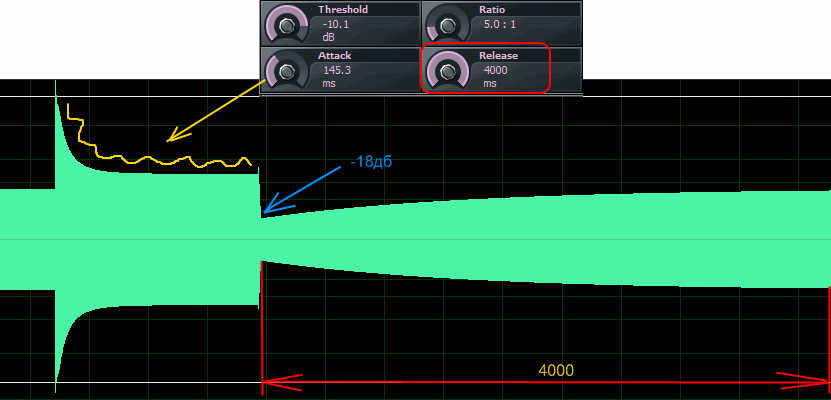
\includegraphics[width=0.75\textwidth]{pic-compress-06}
  \caption{Влияние времени восстановления на форму сигнала}
  \label{pic-compress-06}
\end{figure}

\section{Амплитудная характеристика}
Для отображения параметров инструмента динамической обработки (за исключением времени атаки и времени восстановления) может быть использован график, представляющий зависимость уровня выходного сигнала (вертикальная ось) от уровня входного сигнала (горизонтальная ось).

\begin{figure}[h!]
  \centering
  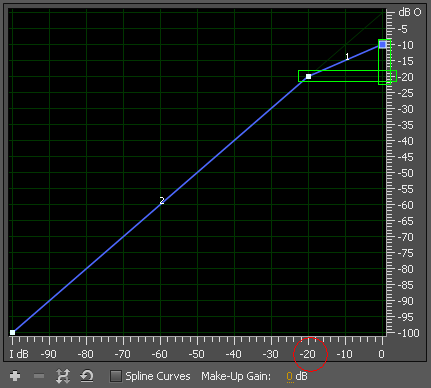
\includegraphics[width=0.75\textwidth]{pic-amp-01}
  \caption{Амплитудная характеристика компрессора}
  \label{pic-amp-01}
\end{figure}

Линия, выходящая из левого нижнего в правый верхний угол, соответствует коэффициенту сжатия 1:1.

Порог (обведен красным цветом) установлен на -20~дБ.

Степень сжатия может быть рассчитана по углу наклона части графика (обведено зеленым цветом): при изменении сигнала на 20дБ (по горизонтали) выходной сигнал изменится на 10~дБ (по вертикали). Таким образом, степень сжатия для данного графика равна 2:1.

На рис. \ref{pic-amp-02}  представлен график более сложного инструмента динамической обработки, сочетающий в себе одновременно компрессор и экспандер.

От первого порога -40~дБ до 0~дБ данное устройство работает как компрессор со степенью сжатия 4:1 (Участок 1).

От второго порога (-70~дБ) до первого~--- как экспандер, степень сжатия 1:1.77 (Участок 2).

Ниже второго порога степень сжатия 1:1 (Участок 3). Максимальный уровень выходного сигнала будет равен -5~дБ.

\begin{figure}[h!]
  \centering
  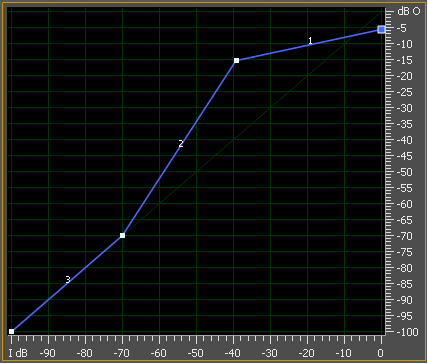
\includegraphics[width=0.75\textwidth]{pic-amp-02}
  \caption{Амплитудная характеристика сложного инструмента динамической обработки}
  \label{pic-amp-02}
\end{figure}

\section{Экспандер, гейт, лимитер}
\textbf{Экспандер} динамического диапазона (\ref{pic-exp-01}) применяют в том случае, когда необходимо расширить динамический диапазон сигнала. Экспандер имеет два порога, при этом обработка происходит между этими двумя порогами.

\begin{figure}[h!]
  \centering
  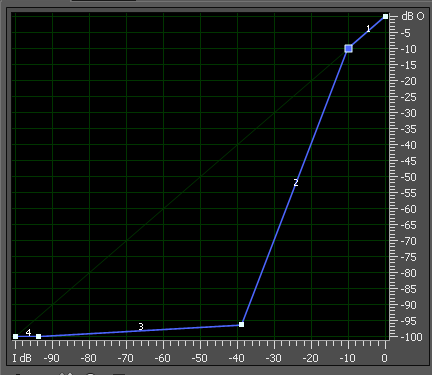
\includegraphics[width=0.75\textwidth]{pic-exp-01}
  \caption{Амплитудная характеристика экспандера}
  \label{pic-exp-01}
\end{figure}

\textbf{Пороговый шумоподавитель} (\emph{гейт}, \emph{noise gate}, \emph{gate})~--- предназначен для подавления сигнала, который находится в заданном динамическом диапазоне.

Однопороговый гейт (рис. \ref{pic-gate-01}) начинает пропускать сигнал (происходит "<открытие"> гейта), как только происходит превышение порога уровнем сигнала, и задерживает сигнал (гейт "<закрывается">), как только уровень сигнала становился бы меньше порога. Двухпороговый гейт (верхний порог~--- \emph{GateOpen}, нижний порог~--- \emph{GateClose}) включается, когда уровень сигнала превысит верхний порог, а выключается только после того, как уровень сигнала станет меньше нижнего порога (рис. \ref{pic-gate-02}).

\begin{figure}[h!]
  \centering
  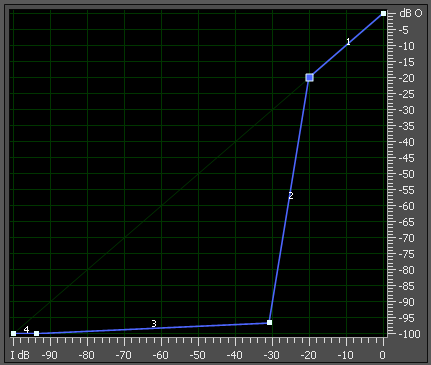
\includegraphics[width=0.75\textwidth]{pic-gate-01}
  \caption{Амплитудная характеристика однопорогового гейта}
  \label{pic-gate-01}
\end{figure}

\begin{figure}[h!]
  \centering
  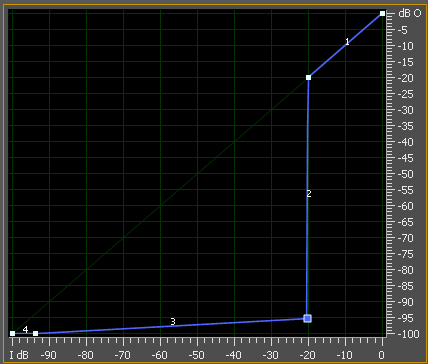
\includegraphics[width=0.75\textwidth]{pic-gate-02}
  \caption{Амплитудная характеристика двухпорогового гейта}
  \label{pic-gate-02}
\end{figure}

\textbf{Лимитер} (\emph{limiter}, ограничитель уровня)~--- ограничитель динамического диапазона, в большинстве случаев используется для предотвращения перегрузки (клипирования) и подавления кратковременных всплесков громкости (пиков), при выравнивании динамики сигнала. В последовательности эффектов лимитер обычно стоит последним.

\begin{figure}[h!]
  \centering
  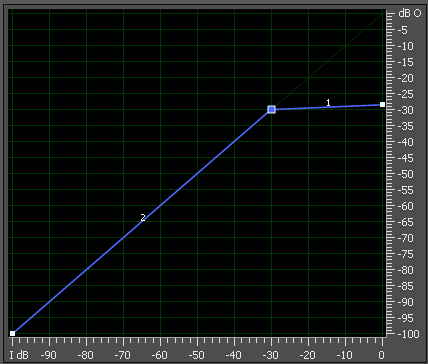
\includegraphics[width=0.75\textwidth]{pic-limiter-01}
  \caption{Амплитудная характеристика лимитера}
  \label{pic-limiter-01}
\end{figure}

\section{Инструменты динамической обработки Adobe Audition}
В составе \emph{Adobe Audition} имеются следующие инструменты динамической обработки:
\begin{itemize}
  \item \emph{Dynamics Processing}~--- универсальная динамическая обработка;
  \item \emph{Hard Limiting}~--- ограничитель уровня;
  \item \emph{Single-band compressor}~--- однополосный компрессор;
  \item \emph{Tube-modeled compressor}~--- инструмент, эмулирующий старые аппаратные устройства-компрессоры;
  \item \emph{Multiband compressor}~--- многополосный компрессор.
\end{itemize}

\subsection{Универсальная динамическая обработка}
Диалоговое окно \emph{Dynamics Processing} открывается командой \emph{Effects > Amplitude And Compression > Dynamics Processing}.
В зависимости от выбранных значений параметров данный эффект может выполнять функции гейта, компрессора, экспандера, лимитера и т.д. Вид обработки и значения параметров можно задавать, редактируя мышью график амплитудной характеристики или вводя точные значения для каждого порога (рис. \ref{pic-dynamic-01}).

\begin{figure}[h!]
  \centering
  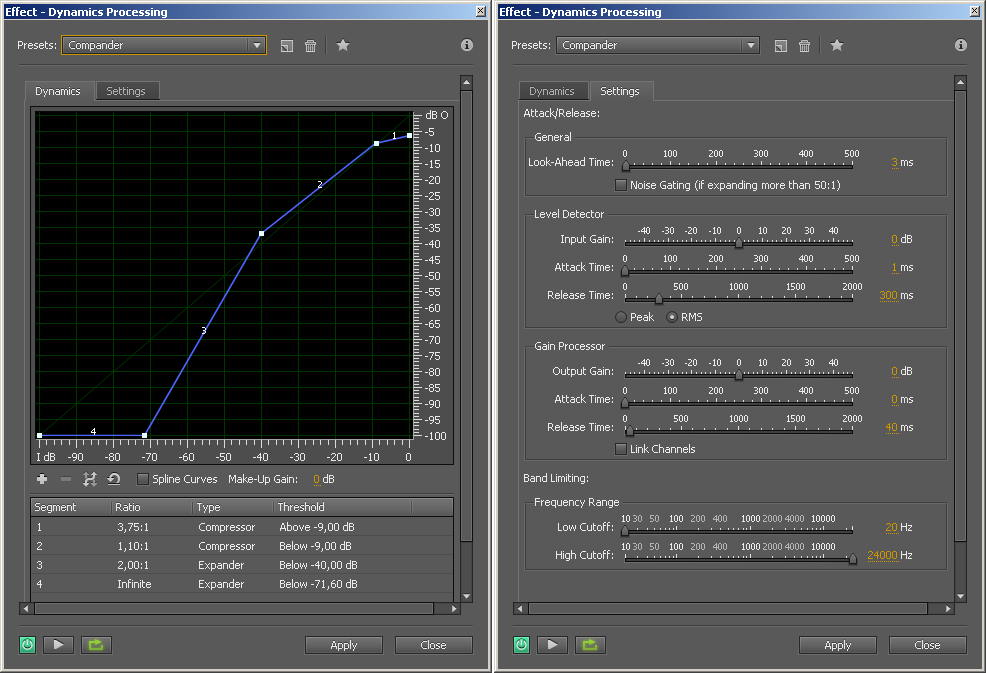
\includegraphics[width=0.95\textwidth]{pic-dynamic-01}
  \caption{Окно инструмента \emph{Dynamics Processing}}
  \label{pic-dynamic-01}
\end{figure}

Диалоговое окно содержит две вкладки:
\begin{itemize}
  \item \emph{Dynamics}~--- позволяет задавать в графическом виде амплитудную характеристику;
  \item \emph{Settings}~--- позволяет настраивать параметры детектора огибающей, процессора усиления и полосы пропускания.
\end{itemize}
	
График амплитудной характеристики редактируется путем задания пороговых точек (добавление~--- щелчок мышью, удаление и точная настройка~--- через контекстное меню точки). Информация о сегментах (значение порога, коэффициент и тип обработки отображается в списке под графиком).

Флаг \emph{Spline Curves} включает режим сглаживания графика.

Параметр \emph{Make-Up Gain} задает величину компенсирующего усиления.

В поле \emph{Lookahead Time} следует задать временной интервал, на который включение устройства динамической обработки должно опережать появление резкого перепада уровня сигнала.

В группе \emph{Level Detector} задаются параметры детектора огибающей, в задачи которого входит определение уровня громкости входного сигнала:
\begin{itemize}
  \item \emph{Input Gain}~--- коэффициент усиления на входе детектора огибающей;
  \item \emph{Attack Time}~--- время атаки;
  \item \emph{Release Time}~--- время восстановления.
\end{itemize}

С помощью переключателей \emph{Peak} и \emph{RMS} вы можете выбрать вид амплитудного детектора~--- пиковый (нежелательно) или среднеквадратический (рекомендуется).

В группе \emph{Gain Processor} задаются параметры контроллера громкости:
\begin{itemize}
  \item \emph{Output Gain}~--- коэффициент усиления на выходе;
  \item \emph{Attack Time}~--- времени атаки;
  \item \emph{Release Time}~--- времени восстановления;
\end{itemize}

Контроллер громкости ослабляет или усиливает сигнал в зависимости от амплитуды, которую определил \emph{Level Detector}.

В группе \emph{Band Limiting} можно задать нижнюю (\emph{Low Cutoff}) и верхнюю (\emph{High Cutoff}) граничные частоты обрабатываемого диапазона. Опции данной группы позволяют подвергать динамической обработке не весь сигнал, а только его отдельные спектральные составляющие. Например, можно задать диапазон от 4352 Гц до 13060 Гц для динамической обработки свистящих звуков в речи человека. Так реализован виртуальный диэсер (\emph{DeEsser}).

\subsection{Ограничитель уровня}
Команда \emph{Effects > Amplitude and Compression > Hard Limiting} открывает диалоговое окно \emph{Hard Limiting} (\ref{pic-limiterau-01}), с помощью которого можно уменьшать до заданного уровня амплитуду звуковых колебаний при условии превышения ею некоторого порога. Амплитуда всех звуковых отсчетов, находящихся ниже этого порога остается неизменной.

\begin{figure}[h!]
  \centering
  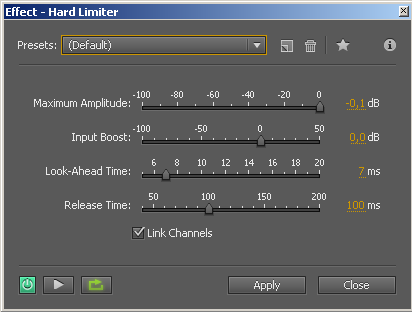
\includegraphics[width=0.75\textwidth]{pic-limiterau-01}
  \caption{Окно инструмента \emph{Hard Limiting}}
  \label{pic-limiterau-01}
\end{figure}

В поле \emph{Maximum Amplitude} задается максимальная допустимая амплитуда волновой формы. Для звука с разрядностью 16 бит рекомендуется устанавливать значение -0.3 дБ.

Перед выполнением ограничения звук может быть предварительно усилен. В поле ввода \emph{Input Boost} задается величина предварительного усиления.

В поле \emph{Look-Ahead Time} нужно задать время упреждения срабатывания ограничителя при появлении пика сигнала. Если значение этого параметра слишком мало, могут появиться слышимые искажения. Рекомендуются значения 4..10 мс.

В поле \emph{Release Time} указывают время, необходимое для восстановления нормального уровня звука после обработки чрезвычайно громкого пика. Для сохранения низкочастотного баса рекомендуется установить значение параметра равным 100 мс.

\subsection{Однополосные компрессоры}
Классический однополосный компрессор (\ref{pic-singleband-01}) реализуется эффектом \emph{Single-band Compressor}. Все параметры задаются при помощи слайдеров:
\begin{itemize}
  \item порог компрессии (threshold);
  \item коэффициент сжатия (ratio);
  \item время атаки (attack);
  \item время восстановления (release);
  \item компенсирующее усиление (output gain).
\end{itemize}

\begin{figure}[h!]
  \centering
  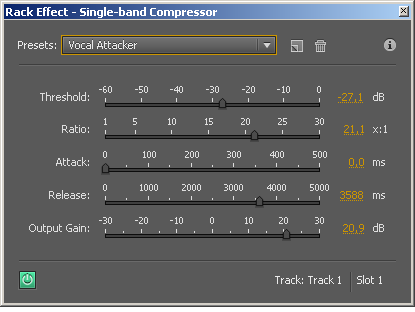
\includegraphics[width=0.75\textwidth]{pic-singleband-01}
  \caption{Окно инструмента \emph{Single-band Compressor}}
  \label{pic-singleband-01}
\end{figure}

Эффект \emph{Amplitude And Compression > Tube-modeled Compressor} имитирует колорит устаревших аппаратных ламповых компрессоров.
Использовать данных эффект можно для того, чтобы добавить (едва заметное) искажение типа \emph{distortion}, которое придаст звуку "<приятную окраску">. Параметры данного эффекта полностью аналогичны настройкам любого другого компрессора.

\begin{figure}[h!]
  \centering
  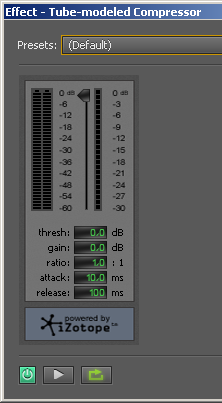
\includegraphics[width=0.3\textwidth]{pic-tubemode-01}
  \caption{Окно инструмента \emph{Single-band Compressor}}
  \label{pic-tubemode-01}
\end{figure}

\subsection{Многополосный компрессор}
Эффект \emph{Amplitude and Compression > Multiband Compressor} позволяет производить независимую компрессию в четырех различных частотных диапазонах. Так как динамика звука для каждого частотного диапазонах уникальна, то данный эффект является мощным средством для сведения звука. Элементы управления данного эффекта (\emph{crossover}: \emph{low}, \emph{mid}, \emph{high}) позволяют задать частоты для кроссовера для разделения звукового сигнала, чтобы затем применить к каждой отдельной полосе собственные параметры компрессии.

\begin{figure}[h!]
  \centering
  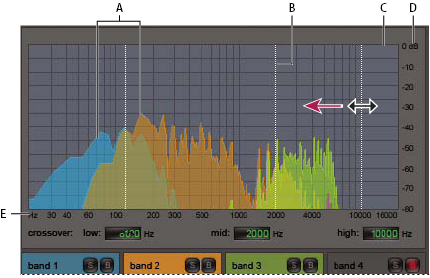
\includegraphics[width=0.75\textwidth]{pic-multiband-01}
  \caption{Окно инструмента \emph{Multiband Compressor}}
  \label{pic-muliband-01}
\end{figure}

Кнопки \emph{Solo} (\emph{S}) позволяют прослушивать полосы по-отдельности, кнопки \emph{Bypass} (\emph{B}) позволяют отключить обработку звука в конкретной полосе частот.

Элементы управления кроссовера:
\begin{itemize}
  \item A. Частотные диапазоны.
  \item B. Маркер кроссовера.
  \item C. Полоса частот, которая не обрабатывается.
  \item D. Шкала громкости.
  \item E. Шкала частот.
\end{itemize}
	
Элементы управления полосой компрессора:
\begin{itemize}
  \item A. Кнопка \emph{Solo}.
  \item B. Кнопка \emph{Bypass}.
  \item C. Настройка порогового уровня.
  \item D. Индикаторы громкости.
  \item E. Индикатор компрессии (ослабления громкости).
\end{itemize}

Индикатор \emph{Gain Reduction} измеряет уровень ослабления сигнала. Чем выше уровень на индикаторе, тем меньше ослабление, которому подвергается сигнал в результате компрессии. Слайдер \emph{С} (\emph{Threshold}) предназначен для настройки порогового уровня, с которого начинается компрессия.

\begin{figure}[ht!]
  \centering
  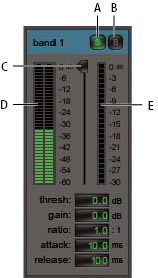
\includegraphics[width=0.3\textwidth]{pic-multiband-02}
  \caption{Секция лимитера инструмента \emph{Multiband Compressor}}
  \label{pic-muliband-02}
\end{figure}

Для компрессии только пиков и большего сохранения динамического диапазона рекомендуется устанавливать порог на 5 дБ ниже максимального уровня громкости; для большей компрессии и большего уменьшения динамического диапазона~--- на 15 дБ ниже уровня пиков.

Параметр \emph{Gain} представляет собой настройку компенсирующего усиления. Диапазон возможных значений: от -18 дБ до +18 дБ. Параметр \emph{Ratio} устанавливает коэффициент компрессии (от 1:1 до 30:1). Параметр \emph{Attack} задает время атаки в милисекундах (от 0 до 500 мсек). Параметр \emph{Release} задает время восстановления (от 0 до 5000 мсек). Параметр \emph{Output Gain} позволяет усиливать или ослаблять результирующий сигнал.

Секция \emph{Limiter}~--- ограничитель уровня, применяется к результирующему сигналу после общего усиления (\ref{pic-muliband-02}).

\section{Инструменты динамической обработки \emph{Waves Platinum Native Bundle}}
\subsection{Waves RComp}
\emph{Waves RComp}~--- компрессор/экспандер, в котором имитируется устройство с традиционным составом элементов управления. 

\begin{figure}[ht!]
  \centering
  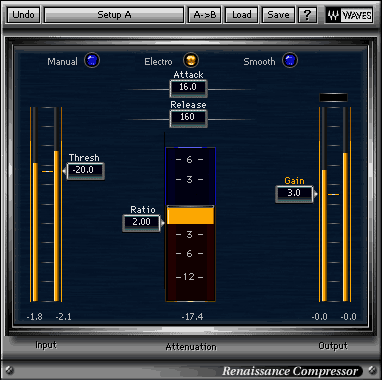
\includegraphics[width=0.75\textwidth]{pic-wavescomp-01}
  \caption{Окно инструмента \emph{RComp}}
  \label{pic-wavescomp-01}
\end{figure}

В левой части окна располагается измеритель уровня входного стереосигнала. 

Значение порога срабатывания прибора устанавливается регулятор \emph{Thresh}. В поле, совмещенном с регулятором, в децибелах отображается уровень порога. По центру окна располагается индикатор текущего уровня сигнала относительно выставленного порога и регулятор степени компрессии/экспандирования \emph{Ratio}. 

Справа располагается измеритель уровня стереосигнала на выходе инструмента, совмещенный с регулятором уровня \emph{Gain}. В полях \emph{Attack} и \emph{Release} настраиваются соответственно время атаки и время восстановления устройства динамической обработки.

\subsection{Waves RDeEsser}
\textbf{Диэсер} представляет собой компрессор, реагирующий на уровень не всего обрабатываемого сигнала, а на уровень его определенных спектральных составляющих. Диэсер получается, когда в канал управления компрессором встраивают фильтр, выделяющий частоты, характерные для свистящих звуков. Наиболее ярким и "<вредным"> представителем последних является звук "<эс">.

\begin{figure}[ht!]
  \centering
  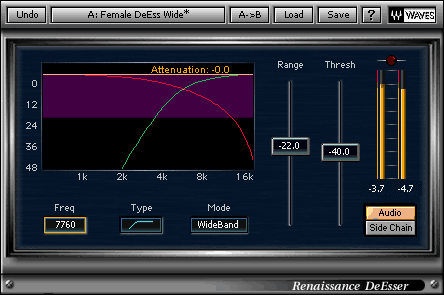
\includegraphics[width=0.75\textwidth]{pic-wavescomp-02}
  \caption{Окно инструмента \emph{RDeEsser}}
  \label{pic-wavescomp-02}
\end{figure}

Если нажата кнопка \emph{Audio}, то на измеритель и на выход плагина поступает обработанный сигнал. При нажатии кнопку \emph{Side Chain}, и вы услышите не то, что получится после обработки, а наоборот то, что в процессе обработки будет из сигнала удалено. Регулируете параметры, слушаете, что получается, и добиваетесь, чтобы слышны были только те неприятные звуки, от которых нужно избавиться. 

Графики позволяют получить визуальное представление о некоторых установленных параметрах деэсера и отображают в режиме реального времени фактическое протекание процесса компрессии.

\subsection{Waves C1 comp, С1 gate}
\emph{C1 comp}~--- один из модулей, составляющих линейку виртуальных приборов динамической обработки. В некоторые более сложные приборы \emph{C1 comp} входит в качестве составной части.

\begin{figure}[ht!]
  \centering
  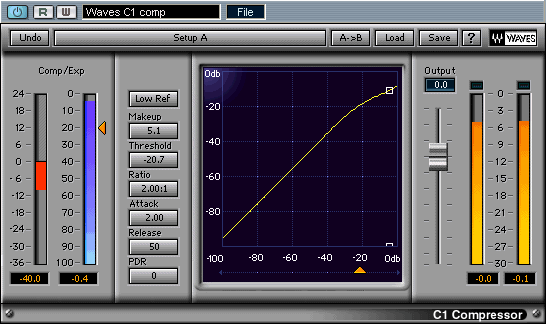
\includegraphics[width=0.75\textwidth]{pic-wavescomp-03}
  \caption{Окно инструмента \emph{C1 Comp}}
  \label{pic-wavescomp-03}
\end{figure}

У графика амплитудной характеристики вместо резкого перегиба в пороговой точке имеется плавный переход, в результате побочные результаты работы устройства становятся менее заметными на слух.

\emph{C1 gate} представляет собой виртуальный прибор динамической обработки, который в зависимости от состояния элементов настройки может выполнять либо функции гейта, либо функции экспандера.

\begin{figure}[ht!]
  \centering
  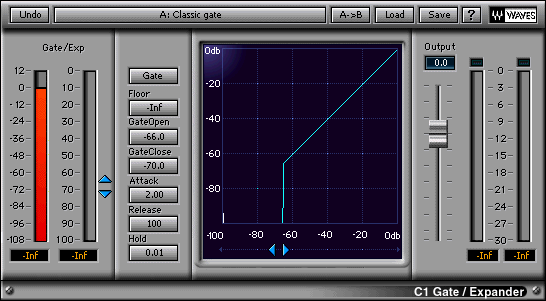
\includegraphics[width=0.75\textwidth]{pic-wavescomp-04}
  \caption{Окно инструмента \emph{C1 gate}}
  \label{pic-wavescomp-04}
\end{figure}

Оба инструмента принадлежат к группе виртуальных приборов динамической обработки C1. Слева находится секция измерителя уровня входного сигнала и измерителя уровня обработки. Далее следует секция элементов управления параметрами обработки, потом координатное поле с интерактивным графиком амплитудной характеристики, связывающим уровни входного и выходного сигналов. В правой части расположен регулятор и измерители уровня выходного сигнала.

Вид обработки выбирается верхней кнопкой. Если она находится в состоянии \emph{Gate}, то плагин становится гейтом, если \emph{Expander}~--- экспандером.

Для того, чтобы избавиться от заметности моментов включения и выключения обработки, предусмотрен постепенный переход от выключенного ко включенному состоянию и обратно. Гейт включается, когда уровень сигнала превысит верхний порог, а выключается только после того, как уровень сигнала станет меньше нижнего порога. Двухпороговый алгоритм позволяет, с одной стороны, надежно отсечь шум в паузах, с другой,~--- сохранить в музыкальных звуках фазу затухания и реверберационные хвосты.

С помощью кнопки-слайдера Floor можно изменять характер динамической обработки сигнала в области перекрытия - на интервале между нижним и верхним порогами. Для классического гейта значение данного параметра составляет "минус бесконечность" (\emph{-Inf}). Это означает, что выключенный гейт как бы настолько ослабляет сигнал, что его уровень становится бесконечно малым, а при включении гейта происходит скачок уровня от \emph{-Inf} до значения, равного пороговому. 

С помощью регулятора \emph{Floor} можно изменить значение коэффициента передачи, соответствующего "<выключенному"> гейту. Он не обязательно должен быть "равен" -Inf.
 
\subsection{Waves RVox}
\emph{RVox} представляет собой гейт, вокальный компрессор и ограничитель, объединенные в одном плагине, управление которым предельно упрощено за счет того, что предусмотрена автоматическая регулировка уровня входного сигнала, а динамические параметры (времена атаки и освобождения) для изменения недоступны.

\begin{figure}[ht!]
  \centering
  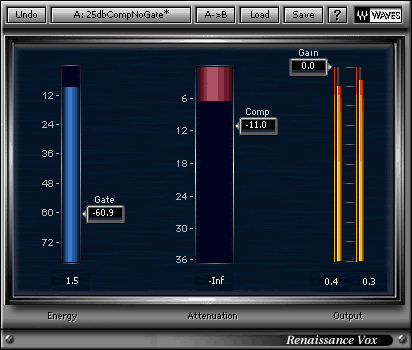
\includegraphics[width=0.75\textwidth]{pic-wavescomp-05}
  \caption{Окно инструмента \emph{RVox}}
  \label{pic-wavescomp-05}
\end{figure}

Инструмент применяет экспандирование для мягкой очистки от шумов в области перекрытия, под которой, вероятно, следует понимать интервал в области низких уровней между порогами включения и выключения гейта. При соответствующем выборе значений параметров плагин хорошо справляется с подавлением шума в паузах.

\subsection{Waves С1 comp/sidechain}
Термин "<\emph{Side Chain}"> переводится как "<боковая цепь">. В данном случае имеется в виду канал управления компрессором, в который могут быть включены дополнительные элементы обработки управляющего сигнала.

Примером полезного применения боковой цепи может служить диэсер, который получается, если в канал управления компрессором включить фильтр, выделяющий частоты, характерные для свистящих звуков. Еще один пример: на вход основного канала компрессора можно подать фоновую музыку, а в канал управления подать сигнал, содержащий речь диктора. Речь без обработки и музыку, обработанную таким компрессором, затем следует смикшировать. В итоге получится, что в паузах музыка будет звучать с нормальной громкостью, а во время разговора будет автоматически приглушаться.

\begin{figure}[ht!]
  \centering
  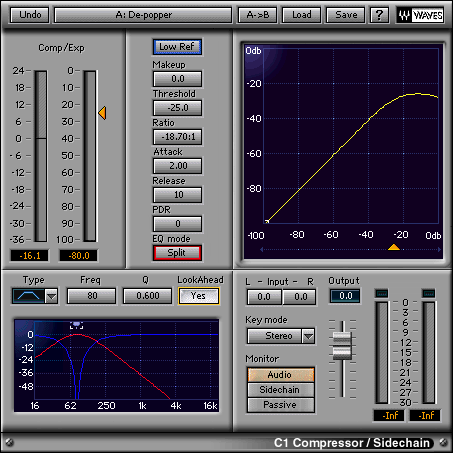
\includegraphics[width=0.75\textwidth]{pic-wavescomp-06}
  \caption{Окно инструмента \emph{С1 comp/sidechain}}
  \label{pic-wavescomp-06}
\end{figure}

Слева вверху располагается секция измерителей, имеющих отношение к уровню входного сигнала, справа вверху~--- координатное поле, совмещенное с регулятором порога. В координатном поле отображается график амплитудной характеристики. 

Элементы, представленные в левой нижней секции, имеют непосредственное отношение к каналу управления. Здесь находится координатное поле с графиками АЧХ кроссовера основного канала и фильтра канала управления, а также все, что требуется для их редактирования.

Новым элементом является кнопка \emph{LookAhead}, которая может находиться в двух состояниях: \emph{No} и \emph{Yes}. Кнопка \emph{Yes} включает алгоритм предсказания. Сначала производится предварительный анализ динамики изменения уровня входного сигнала (особенно важно выявить резкие изменения уровня, а также оценить их величину, время переходного процесса и продолжительность импульсов). За время анализа в соответствии с полученной информацией вырабатывается управляющее воздействие, которое учитывает все выявленные особенности поведения входного сигнала. Если выбраны способы \emph{Split} или \emph{Sidechain}, то управляющий сигнал сначала фильтруют.

\subsection{Waves С1 comp/gate}
\emph{C1 comp-gate}~--- универсальный процессор динамической обработки: компрессор, деэсер, экспандер, гейт, а также сочетание двух приборов, включенных последовательно, и многое другое. Это наиболее полнофункциональный плагин серии \emph{C1}, имеющийся в пакете \emph{Waves Platinum Native Bundle}. Все более простые плагины этой серии входят в него как отдельные модули. Плагин потребляет много ресурсов компьютера, поэтому использовать \emph{C1 comp-gate} нужно только в том случае, когда требуется выполнить комплексную и сложную динамическую обработку сигнала.

\begin{figure}[ht!]
  \centering
  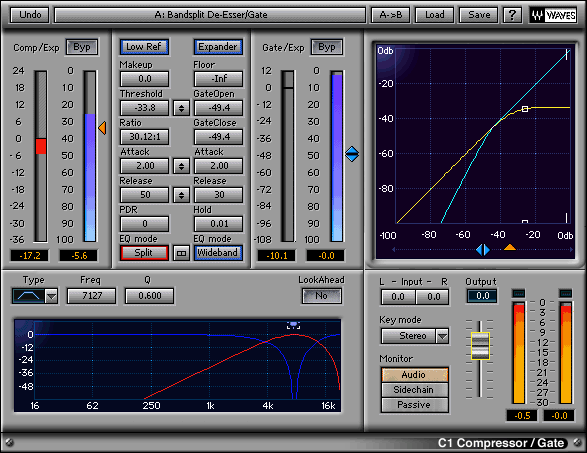
\includegraphics[width=0.75\textwidth]{pic-wavescomp-07}
  \caption{Окно инструмента \emph{С1 comp/gate}}
  \label{pic-wavescomp-07}
\end{figure}

Структурно окно состоит из следующих секций:
\begin{itemize}
  \item измерителей уровней сигналов во входной цепи компрессора/экспандера;
  \item кнопок управления параметрами обоих приборов;
  \item измерителей уровней сигнала во входной цепи гейта/экспандера;
  \item дисплея с координатным полем, предназначенного для отображения графиков амплитудных характеристик;
  \item дисплея с координатным полем, предназначенного для отображения АЧХ фильтров;
  \item коммутаторов, регуляторов и измерителей уровня сигнала на выходе плагина.
\end{itemize}

\section{Примеры динамической обработки}
\subsection{Пример track01}
Часть 1, является качественно записанным на петличный микрофон треком, взятым из документального фильма. Мужская речь имеет неровную динамику, которая могла бы сделать ее трудной для сведения с музыкой или вызвать проблемы в средствах передачи звука с ограниченным диапазоном, таких как телевидение или передача звука по Интернету.

В части 2 трека показан результат умеренной компрессии:
\begin{itemize}
  \item степень сжатия 4:1, порог -15~дБ;
  \item время атаки 1~мсек, время восстановления 300~мсек.
\end{itemize}

В исходном сигнале имеется довольно низкий фоновый шум, но компрессия делает фон сравнительно более громким.

В части 3 трека используется экспандирование для уменьшения фонового шума. Порог выбран так, чтобы быть ниже самых тихих слов говорящего -40~дБ. Атака равна примерно 1,5~мсек, восстановление равно 50~мсек.

В части 4 используется компрессия, сопровождаемая экспандированием (комбинирование обработок для части 2 и части 3). Эта версия придает нашему объекту сильное звучание, делает место съемки чище, и будет более легкой для сведения. Но различия являются тонкими. После ее прослушивания вернитесь к части 1 для сравнения.

\subsection{Пример track02}
Часть 1, является плохо записанным треком документального фильма. При съемке использовался микрофон камеры (почти всегда эта идея является неудачной). Так как объект далеко от микрофона, шум становится громче относительно голоса. Сравнимые расстояния от микрофона до объекта и микрофона до отражающих поверхностей акцентируют эхо помещения.

На первом шаге очистки звука следовало бы использовать эквалайзер для создания провала на резонансных частотах помещения и вырезки шума, а также возвращения некоторой энергии в нижние частоты голоса.

В части 2 показано, как гейт может уменьшить очевидный шум. Порог должен быть ниже самых тихих слов; в этом случае он равен -40~dBFS. Так как гейт работает в широком динамическом диапазоне, то есть  вероятность, что фоновые шумы будут щелкать при быстром включении или выключении.

Внимательно послушайте часть 2. Проблемы помещения понизились в паузах, но все еще остались во время речи объекта. Если бы трек имел умеренное эхо, то этот способ сделал эхо менее назойливым. Если бы эхо было большим, то оно по-прежнему мешало бы разборчивости речи, даже если бы вы полностью отсекли эхо в паузах.

\subsection{Пример track03}
Часть 1, является комментарием к документальному материалу в стиле программы новостей. Хотя диктор выдерживает довольно постоянный уровень, она стремится подчеркивать слова, повышая как громкость, так и тон.

В части 2 исправлено стремление к такому подчеркиванию с помощью компрессора. Порог -12~dBFS, степень сжатия 6:1, атака равна миллисекунде, а восстановление 10мсек. Компенсирующее усиление 4dB.

В части 3 показана предельная степень компрессии. Она разрушает большинство динамики голоса, однако, это может быть полезно при создании спецэффектов или для повышения разборчивости. Степень сжатия 10:1, порог установлен на -20 dB. Атака равна 2 мсек, восстановление - 35мсек. Компенсирующее усиление 10dB.

В части 4 показано воздействие на голос де-эссера. Частоты среза: 4 кГц и 12кГц. Нижние частоты оставлены без изменения, поэтому в голосе не ощущается компрессии. Высокие частоты были обработаны со степенью сжатия 8:1 и с подавлением шипящих звуков, примерно равным -6~дБ. В данном случае, порог был установлен -35~дБ. Атака равна 1мсек, восстановление 5мсек; так обработки коснулись только с высокие частоты, то не было необходимости беспокоится об искажениях из-за слишком малого времени реакции.

\subsection{Пример track04}
Компрессоры, экспандеры и гейты полезны для изменения природы звуковых эффектов, как для достижения высокой реалистичности, так и для создания нереальных, неестественных звуков. Пример демонстрирует применение динамической обработки на примере при записи мортиры.

Часть 1 является оригинальной записью. Мы стоим довольно близко от мортиры и затем слышим далекое эхо.

Часть 2 является результатом компрессии. Хотя звук выстрела остался прежним, он кажется более продолжительным потому, что увеличена первоначальная реверберация. Отдаленное эхо усилено до такой степени, что его звук похож на взрыв снаряда при поражении цели. Сначала эхо было усилено на 10~дБ, а затем к эхо была применена компрессия: степень сжатия 15:1, порог -30~dBFS. Атака равна 3 мсек; восстановление равно 35~мсек. Усиление 18~дБ.

Часть 3 является звуком мортиры, экспандированным ниже порога для того, чтобы оставить только звука выстрела. Без эха это больше похоже на барабан, а не на орудие. Верхний порог -20~dBFS, нижний -40~dBFS. Атака 0.001~мсек, восстановление 50~мсек. Степень сжатия 1:4.

\subsection{Пример track05}
Тот же принцип можно применить и для фоновых звуков. Пример является внутренней атмосферой вагона поезда. Применив небольшую динамическую обработку, вы можете изменить ее характер для более легкого сведения.

Часть 1 является оригинальным звуком. В нем отчетливо слышатся механические шумы.

В части 2 использован компрессор для сглаживания этих шумов. Они остаются, но теперь не будут отвлекать от речи. Степень сжатия равна 10:1, а порог был -10~dBFS, атака была равна 0.5~мсек, а восстановление~--- 35~мсек. При таких значениях низкие частоты искажались бы, но шумы находятся в среднем диапазоне.

В части 3 предпринят другой подход к улучшению пригодности звука для микса. Экспандер с довольно высоким верхним порогом подавляет большинство фона поезда и акцентирует случайные шумы. Верхний порог был равен -10~dBFS, нижний порог был равен -30~dBFS, время атаки и время восстановления оба были равны 10 мсек.

\subsection{Пример track06}
Пример показывает, как динамическая обработка может изменить характер шагов.

Часть 1 является мужскими шагами - кожаные ботинки по деревянному полу.

В части 2 используется экспандер, чтобы превратить ботинки в туфли на высоких каблуках.

Часть 3 является ходьбой в кроссовках по хрустящему бетону.

В части 4 взят эффект хрустящего бетона и использован компрессор, чтобы сделать бетон звучащим "<грязнее">.

\subsection{Пример track07}
Пример показывает, как большое время атаки может изменить характер грохота.

Часть 1 является звуком оркестровой тарелки, по которой ударили палочкой.

Часть 2 является той же записью, только теперь она звучит так, будто по инструменту провели щеткой.

\end{document}

